% lint-skip: 未完成ステータス（figure/table caption 未対応，人手チェック時に解消予定）
\documentclass[../../main.tex]{subfiles}
\begin{document}

\begin{flushright}
  \footnotesize\textit{【自動文字起こし・要確認】}
\end{flushright}

\begin{figure}[htb]
  \centering
  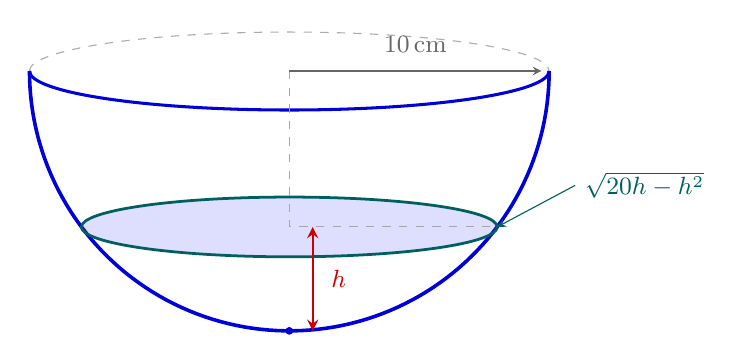
\begin{tikzpicture}[x=0.33cm, y=0.33cm, >=stealth,
    every node/.style={font=\small}]
    % Illustration with h=4 cm: the water-surface radius is 8 cm.
    \coordinate (O) at (0,0);
    \coordinate (Bottom) at (0,-10);
    \coordinate (Surface) at (0,-6);
    \fill[blue!13] (0,-6) ellipse (8 and 1.15);
    \draw[dashed, gray!65] (-10,0) arc[start angle=180,end angle=0,
    x radius=10,y radius=1.5];
    \draw[line width=1.3pt, blue!85!black]
    plot[domain=180:360,samples=100] ({10*cos(\x)},{10*sin(\x)});
    \draw[line width=1.1pt, blue!85!black] (-10,0)
    arc[start angle=180,end angle=360,x radius=10,y radius=1.5];
    \draw[teal!75!black, line width=1pt] (0,-6) ellipse (8 and 1.15);
    \draw[dashed, gray!70] (O) -- (Surface) -- (8,-6);
    \draw[<->, red!80!black, thick] (0.9,-10) -- (0.9,-6)
    node[midway,right=3pt] {$h$};
    \draw[->, gray!80!black] (O) -- (9.7,0)
    node[midway,above=3pt] {$10\,\mathrm{cm}$};
    \draw[<-, teal!75!black] (8,-6) -- (11,-4.4)
    node[right] {$\sqrt{20h-h^2}$};
    \fill[blue!85!black] (Bottom) circle (1.4pt);
  \end{tikzpicture}
  \caption{半球形の容器と水深 $h$ のときの水面の半径}
\end{figure}

\noindent
{\bf [解答]} 時刻 $t$ での水面の面積 $S$, 水深を $h$ とすると, 水の流出速度 $k$ として
\begin{equation}
  -k = S \dfrac{dh}{dt} \quad \cdots \text{①}
\end{equation}
ここで,
\begin{equation}
  S = \pi (20h - h^2) \quad \cdots \text{②}
\end{equation}
又, 題意から,
\[
  -v = \dfrac{dh}{dt}
\]
であり, 両辺積分して, $t=0$ で $h=10$ より,
\begin{equation}
  h = 10 - vt \quad \cdots \text{③}
\end{equation}

\noindent
\paragraph{(1)}

題意の水量 $V(t)$ とすると,
\[
  V(t) = \pi \int_0^{vt} (100 - x^2) dx = \pi \left[ 100x - \dfrac{1}{3}x^3 \right]_0^{vt} = \pi \left( 100vt - \dfrac{1}{3}v^3 t^3 \right) \quad /\!/
\]

\noindent
\paragraph{(2)}

①, ②, ③から
\[
  k = S v = \pi v (20-h) h = \pi v (10+vt)(10-vt) = \pi v (100 - v^2 t^2) \quad /\!/
\]

\newpage

\end{document}
